\documentclass[fleqn]{beamer}

\usepackage[british]{babel}
\usepackage{graphicx,ru,url}
\usepackage{amsmath}
% Use Times for math font and text font.
\RequirePackage[T1]{fontenc}
%\RequirePackage{txfonts}
% bold math must be loaded after Times font
\usepackage{bm}
\usepackage{booktabs} % nice rules (thick lines) for tables
\usepackage{microtype} % improves typography for PDF
\usepackage{xcolor} % Allows colors in fonts
\usepackage{tikz} % Allows creation of tikz pictures
\usepackage{verbatim}
\usetikzlibrary{arrows,shapes,snakes}
\usepackage{hyperref}
%\usepackage{minted} % Allows printing of python (or other) code
% \newminted{python}{fontsize=\scriptsize, 
%     linenos,
%     numbersep=8pt,
%     gobble=4,
%     frame=lines,
%     bgcolor=bg,
%     framesep=3mm}

\setlength{\parindent}{0pt}
\setlength{\parskip}{0pt}
\renewcommand{\baselinestretch}{1.0}

% The title of the presentation:
%  - first a short version which is visible at the bottom of each slide;
%  - second the full title shown on the title slide;
\title[In-Core Neutron Spectroscopy]{
    On Use of Multi-Chambered Fission Detectors for In-Core, Neutron Spectroscopy}

% Optional: a subtitle to be displayed on the title slide
%\subtitle{Show where you're from}

% The author(s) of the presentation:
%  - again first a short version to be displayed at the bottom;
%  - next the full list of authors, which may include contact information;
\author[J. Roberts]{
    Jeremy Roberts}

% The institute:
%  - to start the name of the university as displayed on the top of each slide
%    this can be adjusted such that you can also create a Dutch version
%  - next the institute information as displayed on the title slide
\institute[Kansas State University]{
    Assistant Professor \\
    Mechanical and Nuclear Engineering \\
    Kansas State University}

% Add a date and possibly the name of the event to the slides
%  - again first a short version to be shown at the bottom of each slide
%  - second the full date and event name for the title slide
\date[ANIMMA 2017]{
    ANIMMA 2017 \\
    June 19--23}

\begin{document}
    % These two commands allow bonus slides at the end
    % The bonus slides will not be numbered
    \newcommand{\beginbackup}{
        \newcounter{framenumbervorappendix}
        \setcounter{framenumbervorappendix}{\value{framenumber}}
    }
    \newcommand{\backupend}{
        \addtocounter{framenumbervorappendix}{-\value{framenumber}}
        \addtocounter{framenumber}{\value{framenumbervorappendix}} 
    }
    
    \begin{frame}
        \titlepage
    \end{frame}
    
    \begin{frame}{Fundamental Question}
       \begin{center}
         {\bf\Large Can we unfold a reactor flux spectrum using only a 
         finite set of in-core, fission-detector responses?}
       \end{center}
    \end{frame}
    
    %--------------------------------------------------------------------------%
    \section{Motivation}
    
    \begin{frame}{Small Fission Chambers}
 
        \begin{columns}[c]
            \begin{column}{0.5\textwidth} % split the columns 50/50
              From CEA:
              \begin{itemize}
                \item subminature fission chambers
                \item cylindrical, with radii down to 1.5 mm and 
                      active length of 10 mm
                \item masses of $\approx 10\mu$g
              \end{itemize}
              From K-State:
              \begin{itemize}
                \item micro-pocket fission detectors 
                \item (psuedo) planar, overall radii down to $\approx 6$ mm
                      and active ``length'' of a few mm
                \item masses of $\approx 1\mu$g
              \end{itemize}
            \end{column}
            \begin{column}{0.5\textwidth} % split the columns 50/50
              \begin{center}
                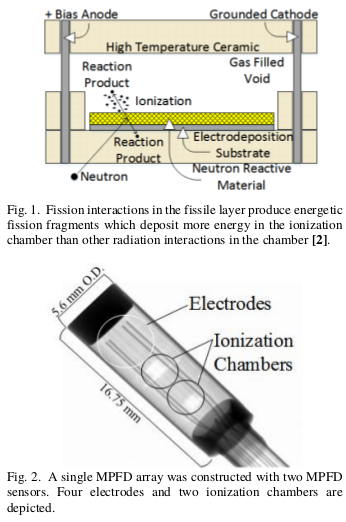
\includegraphics[totalheight=.7\textheight]{mpfd}
              \end{center}
              \tiny  From: Reichenberger, M.A., et al. ``Electronic Support System 
                     Enchnacements for Micro-Pocket Fission Detectors (MPFDs).''
                     IEEE Nucl. Sci. Symp., Strassbourg, FR. 2016.
            \end{column}
        \end{columns}
    \end{frame}
    
    \begin{frame}{Fission Cross Sections (data from http://www.nndc.bnl.gov)}
         \begin{center}
             \includegraphics[totalheight=.8\textheight]{../code/fission_cross_sections.pdf}
         \end{center}
    \end{frame}
    
    
    %--------------------------------------------------------------------------%
    \section{Unfolding Theory}
    
    \begin{frame}{The Assumptions}
      Assume that 
      \begin{itemize}
       \item Only a discrete spectrum (binned or otherwise) is desired
       \item $N$ unique ``responses'' are available
       \item Uncertainties are neglible
       \item The total (integral) flux is known (to be revisited)
      \end{itemize}
    \end{frame}  
    
    
    \begin{frame}{The Constraints}
      With the given assumptions, solve
      \begin{equation}
            r_i = \sum_{g=1}^{G} \Sigma_{f,i,g}  \phi_g\, , 
              \qquad i = 1 \ldots N \, ,
          \label{eq:response}
      \end{equation}     
      or $\mathbf{r} = \bm{\Sigma} \bm{\phi}$, subject to 
      \begin{equation}
            \sum^G_{g=1}{\phi_g} = \phi_{\textrm{tot}} \ .
      \end{equation}
      Here, $N$ will vary while $G = 69$ and $\phi_{\textrm{tot}} = 1$.
    \end{frame}

    
    \begin{frame}{The Solution}
      Equation~\ref{eq:response} is an {\bf inverse problem} (fewer equations than unknowns). 
      \vfill
      Some options: 
      \begin{itemize}
       \item {\bf Minimum norm} \\
             $\bm{\phi} =  \bm{\Sigma}  [\bm{\Sigma} \bm{\Sigma}^T]^{-1}\mathbf{r}$
       \item {\bf Tikhonov} (and other) {\bf regularization} \\
             $\bm{\phi} = [\bm{\Sigma}^T \bm{\Sigma}+ \mathbf{T}^T \mathbf{T}]^{-1} \bm{\Sigma} \mathbf{r}$ (usually $\mathbf{T} = a\mathbf{I}$)
       \item {\bf Maximum entropy} methods
             $\operatorname*{arg\,max}_{\bm{\phi}} S(\bm{\phi}) = 
                \operatorname*{arg\,max}_{\bm{\phi}} \left [ -\sum^G_{g=1} \phi_g \ln(\phi_g) \right ]$ \\
             (variants exist that incorporate prior spectrum + uncertainties)
      \end{itemize}
    \end{frame}
    
    \section{Analysis}
    
    \begin{frame}{Test Spectrum}
         \begin{center}
             \includegraphics[totalheight=.7\textheight]{../code/test_spectrum.pdf}
         \end{center}
         Comments: WIMS 69-group format; fast-to-thermal ratio of 4.
    \end{frame}
    
    \begin{frame}{Multigroup Response Functions}
         \begin{center}
             \includegraphics[totalheight=.85\textheight]{../code/fission_responses.pdf}
         \end{center}
    \end{frame}

    \begin{frame}
       \frametitle{Integral Sensitivities}
    
    \small
        \begin{table}
            \begin{tabular}{llll}
                \toprule
                Isotope & $\sigma_f$ & $\sigma_{f,\text{thermal}}$ & $\sigma_{f, \text{fast}}$ \\ 
                \hline
 ${}^{242m}$Am & 1048.7593 &  4962.9134 &  77.7631\\
 ${}^{245}$Cm & 264.1680 &  1133.7858 &  48.4394\\
 \hline
 ${}^{241}$Pu & 192.7684 &  831.6396 &  34.2817\\
 ${}^{239}$Pu & 179.4585 &  836.1174 &  16.5591\\
 ${}^{233}$U & 106.3772 &  350.3835 &  45.8458\\
 ${}^{235}$U & 85.0867 &  364.1355 &  15.8622\\
 \hline
 ${}^{238}$Pu & 3.1949 &  9.4636 &  1.6398\\
 ${}^{241}$Am & 1.4032 &  4.3195 &  0.6798\\
 ${}^{244}$Cm & 0.7441 &  0.6619 &  0.7645\\
 \hline
 ${}^{240}$Pu & 0.3451 &  0.0498 &  0.4183\\
 ${}^{237}$Np & 0.2358 &  0.0146 &  0.2906\\
 ${}^{234}$U & 0.2256 &  0.0423 &  0.2711\\
 ${}^{242}$Pu & 0.1836 &  0.0090 &  0.2270\\
 \hline
 ${}^{238}$U & 0.0426 &  0.0000 &  0.0532\\
 ${}^{232}$Th & 0.0104 &  0.0000 &  0.0130\\
                \bottomrule
            \end{tabular}
        \end{table}
        
    \end{frame}
    
    \begin{frame}{Some Numerical Details}
     \begin{itemize}
      \item Maximum entropy unfolding based on Sequential Least SQuares Programming
            as implemented in SciPy
      \item All responses, etc., integrated using good old trapezoid rule 
     \end{itemize}

    \end{frame}

    
    
    \begin{frame}{Cases Considered}
      \begin{itemize}
      \item Case 1: ${}^{232}$Th, ${}^{235}$U, ${}^{238}$U
      \item Case 2: Case 1 + ${}^{237}$Np,  ${}^{238}$Pu
      \item Case 3: Case 2 + ${}^{233}$U, ${}^{234}$U, 
                    ${}^{239}$Pu, ${}^{240}$Pu, ${}^{241}$Pu, ${}^{242}$Pu
      \item Case 4: Case 3 +
                    ${}^{241}$Am, ${}^{242m}$Am,
                    ${}^{244}$Cm, ${}^{245}$Cm 
        \begin{itemize}
          \item Vary total flux for maximum entropy unfolding
          \item Compare maximum entropy to minimum norm and Tikhonov
        \end{itemize}
      \pause
      \item \textcolor{red}{Case 5: Case 3 + Cd filters}
      \item \textcolor{red}{Case 6: Case 3 + Gd filters}
      \item \textcolor{red}{Case 7: Case 3 + Cd and Gd filters}
      \end{itemize}
    \end{frame}
    
    \begin{frame}{Unfolded Spectra}
         \begin{center}
             \includegraphics[totalheight=.85\textheight]{../code/reconstructed_flux.pdf}
         \end{center}
    \end{frame}

    \begin{frame}{Unfolded Spectra}
         \begin{center}
             \includegraphics[totalheight=.85\textheight]{../code/reconstructed_flux_lethargy.pdf}
         \end{center}
    \end{frame}
    
    \begin{frame}{Group-Wise, Relative Errors (\%)}
         \begin{center}
             \includegraphics[totalheight=.85\textheight]{../code/groupwise_error.pdf}
         \end{center}
    \end{frame}
    
    \begin{frame}{Group-Wise, Relative Errors (\%, Zoomed)}
         \begin{center}
             \includegraphics[totalheight=.85\textheight]{../code/groupwise_error_zoomed.pdf}
         \end{center}
    \end{frame}
    
    \begin{frame}{Impact of Total Flux Normalization (Errors, \%)}
         \begin{center}
             \includegraphics[totalheight=.85\textheight]{../code/different_total_fluxes.pdf}
         \end{center}
    \end{frame}

    \begin{frame}{Maximum Entropy vs. Minimum Norm and Tikhonov}
         \begin{center}
             \includegraphics[totalheight=.85\textheight]{../code/maxent_vs_minnorm.pdf}
         \end{center}
    \end{frame}  
    
    \begin{frame}{Impact of 0.025 mm Cd Filter on Response Functions}
         \begin{center}
             \includegraphics[totalheight=.75\textheight]{../code/filtered_responses_cd.pdf}
         \end{center}
    \end{frame}  
    
    
    \begin{frame}{Impact of 0.025 mm Gd Filter on Response Functions}
         \begin{center}
             \includegraphics[totalheight=.75\textheight]{../code/filtered_responses_gd.pdf}
         \end{center}
    \end{frame}  
    
    
    \begin{frame}{Case 3 With and Without Filters}
         \begin{center}
             \includegraphics[totalheight=.85\textheight]{../code/filtered_unfold.pdf}
         \end{center}
    \end{frame}  
    
    \begin{frame}{Case 3 With and Without Filters (Zoomed)}
         \begin{center}
             \includegraphics[totalheight=.85\textheight]{../code/filtered_unfold_zoom.pdf}
         \end{center}
    \end{frame}  
    
    \section{Conclusions}
    
    \begin{frame}{The Answer}
       \begin{center}
         {\bf\Large Can we unfold a reactor flux spectrum using only a 
         finite set of in-core, fission-detector responses?}
       \end{center}
       \vfill 
       \pause
       {\bf\Large Yes, to a degree.}
       \begin{itemize}
        \pause
        \item Need Th, U, and Pu to achieve sub-100\%, average, group-wise error
        \pause
        \item Including Am and Cm improves things somewhat
        \pause
        \item Thermal-neutron filtering reduces by half the group-wise error
       \end{itemize}

    \end{frame}
    
        
    \begin{frame}{Moving Forward...}
       ...it would be worth considering:
       \begin{itemize}
        \pause
        \item Advanced unfolding techniques that incorporate prior information (spectrum guess)
              and response uncertainties (counting, mass, composition, etc.)
        \pause
        \item More detailed study of how important each isotope is (e.g., of X responses, which Y would be best?)
        \pause
        \item More detailed study of filters (this was a hotel-room study)
        \pause 
        \item A sanity check regarding whether any of this is actually doable in practice
       \end{itemize}
       \vfill 
       \pause 
       \begin{center}
        {\bf Thanks!  Questions? \\
        jaroberts@ksu.edu}
       \end{center}


    \end{frame}
   % \backupend % Ends the non-numbered slides
    
\end{document}
